\documentclass[a4paper,12pt]{article}
\usepackage[a4paper, total={6in, 8in}]{geometry}
\usepackage[english]{babel}
\usepackage[protrusion=true,
            expansion=true,
            final,
            babel
                ]{microtype}
\usepackage{graphicx} % Required for inserting images
\usepackage{setspace}
\usepackage{parskip}
\usepackage{amsmath}
\usepackage{amsthm}
\usepackage{amssymb}
\usepackage{hyperref}
\theoremstyle{definition}
\newtheorem{definition}{Definition}[section]
\newtheorem{theorem}{Theorem}[section]
\newtheorem{corollary}{Corollary}
\newtheorem{lemma}[theorem]{lemma}
\usepackage{float}
\newcommand{\signed}[1]{%
  {\unskip\nobreak\hfil\penalty50
   \hskip2em\hbox{}\nobreak\hfil#1
   \parfillskip=0pt \finalhyphendemerits=0 \par}
}


\hypersetup{
    colorlinks=true,
    linkcolor=blue,
    citecolor=red,
    filecolor=magenta,      
    urlcolor=cyan,
    pdftitle={Overleaf Example},
    pdfpagemode=FullScreen,
}
    
\begin{document}
\graphicspath{{./images}}

\begin{center}
    \doublespacing
    {\Large \textbf{King Fahd University of Petroleum and Minerals} }\\ 
    {\large \textbf{
    College of Computing and Mathematics\\
    Mathematics Department 
    } } 
\end{center} 

\begin{figure}[h]
    \centering
    
\includegraphics[width=200px]{KFUPM_LOGO}
\end{figure}

\begin{center}\onehalfspacing
    \Large \textbf{Math 619-Project}\\
    \normalsize \textbf{Term 231} \\
    \Large \textbf{Progress Report}\\
    \textbf{Project}: Deep Learning Methods for Partial Differential Equations (PDEs)
\end{center}
\vspace{1em}
\large
\begin{center}
\bgroup
\def\arraystretch{1.3}
\begin{tabular}{|c|c|}
    \hline
    \textbf{Name} & \textbf{KFUPM ID} \\
    \hline
    Hashim Al-Sadah & 201578370\\
    \hline
    Abdulwahab Alghamdi & 201734070\\
    \hline
    Hussain Al-Sinan & 202205120\\
    \hline 
\end{tabular}
\egroup
\end{center}
\vspace{1em}
\begin{center}
    \textbf{Instructor:} Dr. Jamal Al-Smail
\end{center}
\normalsize


\onehalfspacing % for double spacing, comment if ypu don't want to
\section*{Abstract}
Partial differential equations (PDEs) are essential components for modelling different processes 
and systems in various scientific and engineering areas. To predict the behavior of a certain system, 
one needs to solve or simulate the PDEs that describe that system. However, 
obtaining an analytical solution to PDEs is a difficult task in most practical situations, 
especially in the case of nonlinear or high dimensional PDEs. 
Due to the rapid evolution and advancements in the field of deep learning, 
researchers are starting to use deep neural networks (DNN) to approximate the solution of PDEs. 
Different models have been developed to perform this task such as Physics-Informed Neural Networks (PINNs) 
and Neural Operator. The speed and the efficiency of these models can surpass other common solvers 
such as Finite Elements (FM), Finite Difference (FD), and spectral methods in certain cases. 
In this project, we will utilize these deep learning models to solve an industry-related problem that 
requires PDEs approximation and compare the accuracy of the used method against 
experimental or simulated data obtained through other available solvers.

\section{Introduction}
Due to the increase power of computation and the success of deep learning models to 
solve different problems in various fields such
as computer vision\cite{chai2021deep}, pattern recognition\cite{serey2023pattern}, 
and natural language and speech processing\cite{NLPChai}, 
researchers were inspired to apply deep neural network to solve problems in the field of scientific computing. 
One of the common and challenging problems is the problem of solving partial differential equations (PDEs).
Different systems and processes are modelled by PDEs whether it is a natural system such as 
modelling a biological or a physical phenomena\cite{grossmann2023can,beck2020overview}, or whether it is not a natural system such as
simulating socioeconomic or financial models\cite{beck2020overview}. Deep learning-based PDEs solver surpass classical methods such as 
finite element or finite difference in certain cases\cite{grossmann2023can}. 
One of them is the case of high dimensional PDEs since classical solvers require discretizing the PDEs' domain into a mesh, 
which causes the number of computations to increase exponentially with the increase of the dimensions and this is known as the curse of dimensionality. 
On the other hand, deep learning models are mesh-free models, and they only require training data from the PDEs domain. 
Other situations where deep neural networks exceeds the traditional solvers is when the PDE is 
nonlinear or non-smooth, which makes it difficult to discretize\cite{grossmann2023can}. 

Physics-informed Neural Network (PINN) is the most basic and widely used model for approximating PDEs' solutions. 
PINN is unsupervised learning model since it does not require any 
labelled data to learn the approximated function or solution\cite{cuomo2022scientific}.
Despite being unsupervised technique, it is possible to include experimental data along with the physical prior knowledge
in order to guide the neural network to the optimal approximation by reducing the 
number of admissible solutions to the problem\cite{hao2022physics,raissi2019physics}.
Similar to the fully connected neural network, the physics-informed neural network consists of 
an input layer, hidden layers, and an output layer. First, the input layer is used to feed 
the training data into the neural network.  Then, the hidden layers map the data to higher dimensions though 
a series of linear transformation followed by a nonlinear activation function. 
Finally, the hidden layers map the data to the output layer, which provides the output of the approximated function. 
The physics-informed neural network (PINN) updates the learning parameters by minimizing a loss function that takes 
into account the losses due the boundary and initial conditions as well as the PDEs' residual. 
After the training process, the neural network should be able to approximate a function that obeys the laws provided by the PDEs. 
Therefore, the procedure of including the PDEs' residual helps to restrict the number of possible solutions\cite{cuomo2022scientific}. 

Another famous model, which has been developed recently, is the Neural Operator model. 
What makes neural operators different from physics-informed neural networks (PINNs) is that the former 
learns a mapping between infinite function spaces unlike PINN where the mapping occurs between finite spaces or sets. 
This enables neural operators to learn an operator instead of a function and hence the name Neural Operator.
The key difference between PINN and neural operators in terms of architecture is that the 
hidden layers in neural operators consist of linear operators, usually integral operators, 
followed by a nonlinear activation function. 
Therefore, neural operators are considered a generalization of physics-informed neural network\cite{kovachki2021neural}.

Overall, deep learning methods for PDEs are powerful solvers. 
They have the potential for resolving various problems and challenges faced by the classical methods. 
The advantage of neural networks models is that they are mesh-free methods, which enables them to approximate 
the solution for nonlinear, non-smooth, and high dimensional PDEs without suffering from the cures of dimensionality.
Furthermore, they utilize the algorithm of automatic differentiation to compute the residual of the PDEs. 
The algorithm is implemented by the majority of deep learning libraries, 
which makes the overall implementation process simple and easy. 

\section{PINN}
In this section, we develop some mathematical notation to use throughout the project, 
and discuss the procedure of approximating ordinary and partial differential equations. All the 
codes that have been used in this section will be available on the GitHub repository 
\url{https://github.com/HashimAlSadah/MX-Project.git}.

\subsection{Overview}
Let us first consider a general nonlinear differential equation
\begin{equation}\label{general_PDE}
\begin{aligned}
\mathcal{F}(u, \gamma)(\mathbf{x}) = f(\mathbf{x}) \qquad \mathbf{x} \in  \Omega,\\
\mathcal{B}(u, \gamma)(x, t) = g(t) \qquad x \in \partial{\Omega}, \\
\mathcal{I}(u, \gamma)(x, t_0) = h(x) \qquad x \in \partial{\Omega_0}
\end{aligned}
\end{equation}

Where $u(\mathbf{x})$ is the unknown function that we are trying to approximate, 
$\mathbf{x} = [ x_1, x_2, \dots, x_{d-1}, t]$ is the vector of space and time 
in the domain $\Omega \subset \mathbb{R}^d$  with boundary $\partial{\Omega}$, 
$\gamma$ are parameters related to the problem, $\mathcal{F}$ is the nonlinear 
differential operator, $\mathcal{B}$ is the boundary conditions, $\mathcal{I}$ is 
the initial conditions, and $f(\mathbf{x})$, $g(t)$, and $h(x)$ are specified 
functions for a certain problem. 

Since it is established that multilayer feedforward neural networks 
are universal function approximators\cite{hornik1989multilayer}, it means that 
a neural network with at least one hidden layer can approximate a function 
from a finite dimensional set to another with 
any arbitrary error given that we use a sufficient number of hidden neuron or units.

\subsection{Universal function approximator theorem}
In this part, we explore the theoretical aspects of the universal approximator theorem.
For this part we will follow the definitions and the theorems as stated in the paper 
by Hornik et al. (1988) and we try to elaborate and explain as much as possible. 

We start by introducing the necessary definitions before stating any theorems.


\begin{definition}\label{affine def}
    For any $r \in \mathbb{N}$, $\mathbf{A}^r$ is the set of all affine functions 
    from $\mathbb{R}^r$ to $\mathbb{R}$. In other words, it is the set of all functions
    $A(\mathbf{x}) = \mathbf{w} \cdot \mathbf{x} + b$. Where $\mathbf{x, w} \in \mathbb{R}^r$
    and $b \in \mathbb{R}$.  \signed{$\square$}
\end{definition}


The affine transformation in Definition \ref{affine def} represents the output of one hidden 
units before applying any activation function. $\mathbf{x}$ represents the input to the neural 
network, $\mathbf{w}$ represents the weights between the input and a particular hidden unit, and
$b$ is the bias term. 

\begin{definition}\label{class of NN}
    For any Borel measurable function $G(\cdot)$ mapping $\mathbb{R}$
    to $\mathbb{R}$ and $r \in \mathbb{N}$ define $\sum^r(G)$ to be the class of 
    functions  
    \begin{multline*}
    \biggl\{f: \mathbb{R}^r \rightarrow \mathbb{R} 
    \, \bigg| \, f(x) = \sum_{j=1}^{q} \beta_j G(A_j(\mathbf{x})), 
    \mathbf{x} \in \mathbb{R}^r, \beta_j \in \mathbb{R},
    \\[-0.75em] \mathbf{A}_j \in \mathbf{A}^r,
    \quad j = 1, 2, \dots
    \biggr\} \; \square
    \end{multline*}
\end{definition}

When the function $G$ is a squashing (activation) function, the class of 
functions in Definition \ref{class of NN} becomes the class of neural network 
with one hidden layer with $q$ hidden units. $\beta_j$ are the weights from the 
hidden layer to the output of the neural network. Next, we define what a 
squashing (activation) function is.

\begin{definition}\label{general class NN}
    A function $\Psi : \mathbb{R} \rightarrow [0, 1]$ is a squashing function if 
    \begin{enumerate}
        \item It is non-decreasing function.
        \item $\lim_{\lambda \rightarrow \infty} \Psi(\lambda) = 1$
        \item $\lim_{\lambda \rightarrow -\infty} \Psi(\lambda) = 0$
    \end{enumerate}
    for all $\lambda \in \mathbb{R}$. \signed{$\square$}
\end{definition}

\begin{definition}
    For any Borel measurable function $G(\cdot)$ mapping 
    from $\mathbb{R}$ to $\mathbb{R}$ and $r \in \mathbb{N}$, 
    define $\sum \prod^r (G)$ to be the class of functions 
    \begin{multline*}
        \biggl\{ f: \mathbb{R}^r \rightarrow \mathbb{R} \, \bigg| \, 
        f(\mathbf{x}) = \sum_{j=1}^{q} \beta_j \cdot \prod_{k=1}^{l_j} G( A_{jk}(\mathbf{x})), 
        \, \mathbf{x}^r \in \mathbb{R}, \beta_j \in \mathbb{R}, \\[-0.75em] 
        \mathbf{A}_j \in \mathbf{A}^r, \quad j = 1, 2, \dots
        \biggr\} \; \square
    \end{multline*} 
\end{definition}

The class of functions defined in Definition \ref{general class NN} 
is more general class of feedforward neural network, so proving that 
$\sum\prod$ is a class of universal functions approximators is sufficient 
to show that the same apply to the class $\sum$ since the latter is a special 
case of the earlier, which can be obtained by setting $l_j = 1$ for all $q$. 

\begin{definition}\label{continuous-measurable funs}
    Define $C^r$ to be the set of all continuous functions mapping from 
    $\mathbb{R}^r$ to $\mathbb{R}$ and $M^r$ to be the set of all measurable
    functions mapping from $\mathbb{R}^r$ to $\mathbb{R}$. Also, denote the 
    Borel $\sigma$-field of $\mathbb{R}^r$ by $B^r$. \signed{$\square$}
\end{definition}

Therefore, by Definition \ref{continuous-measurable funs}, if $G$ is any continuous 
function, then the classes $\sum^{r}(G)$ and $\sum\prod^{r}(G)$ belong to $C^r$. Similarly,
if $G$ is any Borel measurable function, then the classes $\sum^{r}(G)$ and $\sum\prod^{r}(G)$
belong to $M^r$. 

\textbf{Note:} If a function is continuous then it is measurable, but the converse is 
not true in general.

The closeness of functions $f, g \in C^r$  or $f, g \in M^r$ is measured by 
some metric $\rho$ on $C^r$ or $M^r$. The closeness of one class of functions 
to another is measured by the concept of denseness, which will be defined next.

\begin{definition}\label{denseness def}
    A subset $S$ of a metric space $(X, \rho)$ is $\rho$-dense in
    a subset $T$ if for every $\epsilon > 0$ and for every $t \in T$ 
    there exists $s \in S$ such $\rho(s, t) < \epsilon$. \signed{$\square$}
\end{definition}

Definition \ref{denseness def} implies that an element of $S$ can approximate 
an element of $T$ to any desired degree of accuracy. In our case, $X$ and $T$ 
represent $C^r$ or $M^r$, and $S$ represents $\sum^{r}(G)$ or $\sum\prod^{r}(G)$.

Before introducing the main theorem, we need one last definition since we would 
like to show that $\sum^{r}(G)$ and $\sum\prod^{r}(G)$ are uniformly dense on 
a compacta in $C^r$ or $M^r$.

\begin{definition}
    A subset $S$ of $C^r$ is uniformly dense on a compacta in $C^r$
    if for every compact subset $K \subset \mathbb{R}^r$ S is $\rho_K$-dense
    in $C^r$. Where 
    $$\rho_K(f, g) \equiv sup_{x \in K} \left| f(x) - g(x) \right|, 
    \quad \text{for all } f, g \in C^r
    $$
    A sequence of functions ${f_n}$ converges to a function $f$ 
    uniformly on compacta if for all compact $K \subset \mathbb{R}^r$
    $\rho_K(f_n, f) \rightarrow 0$ as $n \rightarrow \infty$. 
    \signed{$\square$} 
\end{definition}

\begin{theorem}
    Let $G: \mathbb{R} \rightarrow \mathbb{R}$ be any continuous non-constant 
    function. Then $\sum\prod^r(G)$ is uniformly dense on compacta in $C^r$.
    \signed{$\square$}
\end{theorem}
Which says that \(\sum \prod (G)\) that is the feed-forward network is capable of accurately approximating any real-valued continuous function over a compact set. \cite{hornik1989multilayer}
\newpage
\subsection{Training PINN}
Therefore, the target function $u(\mathbf{x})$ can be approximated with a neural network,
$$
u_{\theta}(\mathbf{x}) \approx u(\mathbf{x})
$$ 
Where $\theta$ represents the parameters of the neural network, which consists of
weights and the biases.

As stated earlier, a neural network is composed of input layer, 
hidden layers, and output layer. Therefore, neural network with $L$
layers can represent $u_\theta$ as a compositional function as the following.
$$
u_{\theta}(\mathbf{x}) = f_L(\mathbf{x}) \circ f_{L-1}(\mathbf{x}) \circ \dots \circ f_1(\mathbf{x})
$$
But each layer consists of a linear transformation and a nonlinear scalar activation function
$$
f_i(\mathbf{x}) = \sigma_i \left( \mathbf{W}_i \cdot \mathbf{x}_i + \mathbf{b}_i \right), 
$$
Denote the linear transformation by $T(\mathbf{x})$
$$
T(\mathbf{x}) = \mathbf{W}_i \cdot \mathbf{x}_i + \mathbf{b}_i 
$$
Therefore, 
\begin{equation}
u_{\theta}(\mathbf{x}) = T_L \circ \sigma \circ T_{L-1} \circ \dots \circ \sigma \circ T_1
\end{equation}
We are assuming that the same activation function $\sigma$ is used for all the layers.

PINN converts the problem of solving a differential equation 
to an optimization problem since PINN attempts to determine the parameters $\theta$ 
that approximate the function $u$ by minimizing a loss function $\mathcal{L}(\theta)$\cite{cuomo2022scientific}.

The loss function includes the partial differential equation, initial and boundary conditions, and 
the labeled data if available.
\begin{equation}
\mathcal{L}(\theta) = w_{\mathcal{F}} \mathcal{L}_{\mathcal{F}}(\theta)
+ w_{\mathcal{B}} \mathcal{L}_{\mathcal{B}}(\theta) 
+ w_{\mathcal{I}} \mathcal{L}_{\mathcal{I}}(\theta)
+ w_{\mathcal{D}} \mathcal{L}_{\mathcal{D}}(\theta)
\end{equation}
Where $\mathcal{L}_{\mathcal{F}}(\theta)$, $\mathcal{L}_{\mathcal{B}}(\theta)$, 
$\mathcal{L}_{\mathcal{I}}(\theta)$, and $\mathcal{L}_{\mathcal{D}}(\theta)$ are the differential equation loss,
boundary conditions loss, initial conditions loss, and labeled data loss, respectively, and $w_{\mathcal{F}}$, 
$w_{\mathcal{B}}$, $w_{\mathcal{I}}$, and $w_{\mathcal{D}}$ are their corresponding weights. 
The weights for the losses are usually hyperparameters specified manually.

Considering the loss function to be the mean square error function, then the losses can be 
defined as the following.
\begin{equation}\label{pde loss}
\mathcal{L}_{\mathcal{F}}(\theta) = MSE_{\mathcal{F}} 
= \frac{1}{N_c} \sum_{i=1}^{N_c} \bigg| \mathcal{F}(u_\theta)(\mathbf{x}_i) - f(\mathbf{x}_i) \bigg|^2
\end{equation}
Where $N_c$ are the collocation points, which are points within the domain $\Omega$

(\ref{pde loss}) is formulated as above since we are requiring the left-hand side of 
$$
\mathcal{F}(u)(\mathbf{x}) = f(\mathbf{x})  \Rightarrow 
\mathcal{F}(u)(\mathbf{x}) - f(\mathbf{x}) = 0
$$
to be zero.

Similarly, for $\mathcal{L}_{\mathcal{B}}(\theta)$,  $\mathcal{L}_{\mathcal{I}}(\theta)$, and 
$\mathcal{L}_{\mathcal{D}}(\theta)$.
\begin{equation}\label{boundary loss}
\mathcal{L}_{\mathcal{B}}(\theta) = MSE_{\mathcal{B}} 
= \frac{1}{N_b} \sum_{j=1}^{N_b} \bigg| \mathcal{B}(u_\theta)(x, t_j) - g(t_j) \bigg|^2
\end{equation}
\textbf{Note:} (\ref{boundary loss}) shows the boundary condition loss for one point in space $x$ 
at different time $t_j$. 

\begin{equation}
\mathcal{L}_{\mathcal{I}}(\theta) = MSE_{\mathcal{I}} 
= \frac{1}{N_i} \sum_{i=1}^{N_i} \bigg| \mathcal{I}(u_\theta)(x_i, t_0) - h(x_i) \bigg|^2
\end{equation}

\begin{equation}
\mathcal{L}_{\mathcal{D}}(\theta) = MSE_{\mathcal{D}} 
= \frac{1}{N_d} \sum_{i=1}^{N_d} \bigg| u_{\theta}(\mathbf{x}_i) - u_i \bigg|^2
\end{equation}
Where $u_i$ is a labeled example or data.

\subsection{Continuous model}
\subsubsection{Linear PDE example}
To demonstrate the ability of PINN to approximate the solution of a PDE, we 
consider the following heat or diffusion equation.
\begin{equation}
\frac{\partial u}{\partial t} = \frac{\partial^2 u}{\partial x^2}
- e^{-t} \sin{(\pi x)} (1 - \pi^2), \quad -1 < x < 1, \quad 0 < t \le 1
\end{equation} 
Subject to the following boundary conditions
\begin{equation}
    u(x=-1, t) = u(x=1, t) = 0
\end{equation}
and the initial condition
\begin{equation}
u(x, t=0) = \sin(\pi x)
\end{equation}

The exact solution for the problem is 
\begin{equation}
u(x, t) = e^{-t} \sin(\pi x), \quad -1 \le x \le 1, \quad 0 \le t \le 1
\end{equation}

To solve the problem, we have discretized the x-axis and the time into $30$ points each.
Therefore, our loss functions will be the following
$$
\mathcal{L}_{\mathcal{F}} = \frac{1}{900} \sum_{i=1}^{30} \sum_{j=1}^{30} 
\Bigg| 
\frac{\partial u_\theta}{\partial t}\bigg|_{x_i, t_j} - \frac{\partial^2 u_\theta}{\partial x^2}\bigg|_{x_i, t_j}
+ e^{-t_j} \sin{(\pi x_i)} (1 - \pi^2) 
\Bigg|^2
$$

$$
\mathcal{L}_{\mathcal{B}_1} = \frac{1}{30} \sum_{j=1}^{30} 
\Bigg| u_\theta(x=-1, t_j) \Bigg|^2, \qquad
\mathcal{L}_{\mathcal{B}_2} = \frac{1}{30} \sum_{j=1}^{30} 
\Bigg| u_\theta(x=1, t_j) \Bigg|^2,
$$

$$
\mathcal{L}_{\mathcal{I}} = \frac{1}{30} \sum_{i=1}^{30}
\Bigg| u_\theta(x_j, t=0) - \sin(\pi x_j) \Bigg|^2
$$

The used neural network consists of $4$ hidden layers and $10$ hidden units or neurons.
The learning rate was set to be $0.0001$, and we used Adam optimizer, which utilizes the 
algorithm of stochastic gradient descent. 

\begin{figure}[H]
    \centering
    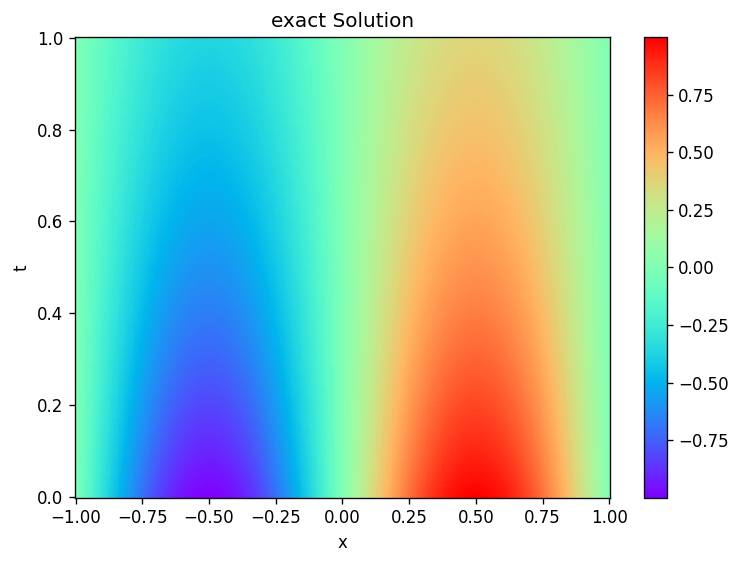
\includegraphics[width=250px]{images/exact_solution_diff.png}
    \vspace{-1em}
    \caption{Exact solution $u(x,t)$}
    \label{exact diff}
\end{figure}

\begin{figure}[H]
    \centering
    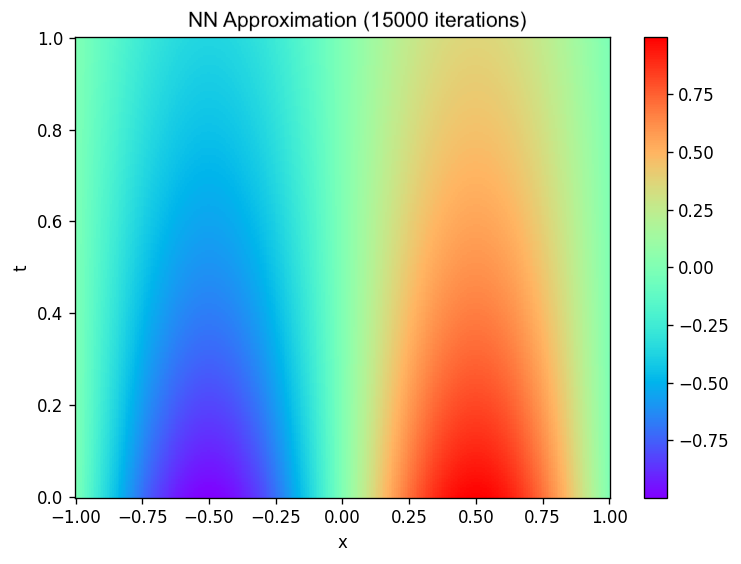
\includegraphics[width=250px]{images/approx_solution_diff.png}
    \vspace{-1em}
    \caption{Approximated solution $u_\theta(x,t)$}
    \label{approximation diff}
\end{figure}

\begin{figure}[H]
    \centering
    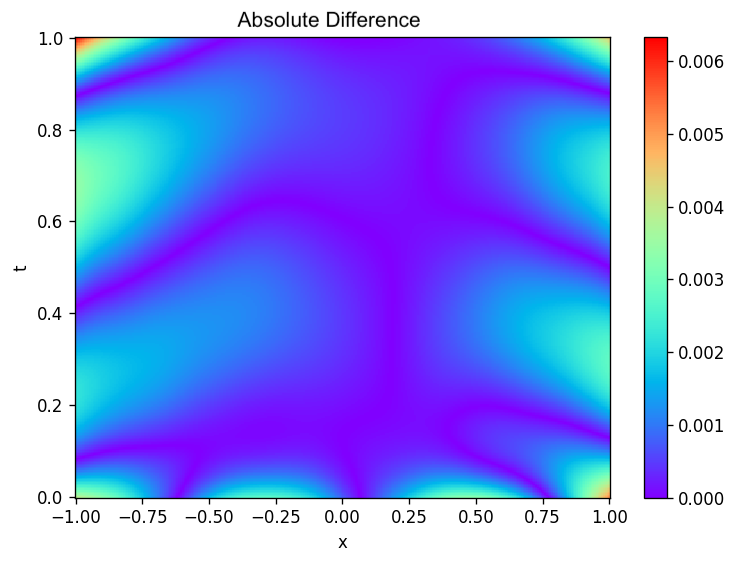
\includegraphics[width=250px]{images/difference_diff.png}
    \vspace{-1em}
    \caption{Absolute difference between $u_(x,t)$ and $u_\theta(x,t)$}
    \label{absolute diff}
\end{figure}

Figure \ref{absolute diff} shows the difference between the exact solution 
in Figure \ref{exact diff} and the neural network approximation in Figure \ref{approximation diff}
where it indicates a global error of order $10^-2$ after 15000 iterations. The code and the simulation
details are on \href{https://github.com/HashimAlSadah/MX-Project/blob/main/PINN/continuous_time_model/PDE_diffusion_PINN.ipynb}
{GitHub}.

\subsubsection{Nonlinear PDE example}
Consider the following nonlinear PDE, Burgers' equation
\begin{equation}
\frac{\partial u(x,t)}{\partial t} 
= -u(x,t)\frac{\partial u(x,t)}{\partial x} 
+ \nu \frac{\partial^2 u(x,t)}{\partial x^2}, \quad x \in [-1, 1], \quad t \in [0, 1]
\end{equation}
Where $\nu$ is the diffusion coefficient. For our example, we will use $\nu = 0.01 / \pi$.

The PDE is subject to the following initial and boundary conditions.
\begin{equation}
\begin{aligned}
&u(x, 0) = -sin(\pi x), \\
&u(-1, t) = u(1, t) = 0
\end{aligned}
\end{equation}

\textbf{Reference solution}\\
It is possible to obtain the analytical solution for Burgers equation for a 
restricted set of initial conditions functions, $u(x,t=0) = g(x)$. This can be done by 
using the Cole-Hopf transformation, which is a nonlinear transformation\cite{kutluay1999numerical}.
\begin{equation}
u(x, t) = -2 \nu \frac{\theta_x}{\theta} = -2 \nu \log[\theta(x,t)]
\end{equation}
This transformation turns the nonlinear Burgers PDE into the heat equation
\begin{equation}
\theta_t = \nu \theta_{xx}
\end{equation}
For the purpose of making the code general when changing the initial conditions (or even the boundary conditions), 
we are going to use the explicit finite difference (conditionally stable) to approximate the solution for 
Burgers equation and that approximation will be our reference solution.

\textbf{Finite difference discretization}\\
We will discretize the x-dimension into $n$ sub-intervals with $n+1$ points using a step size of $\Delta x = h$
$$
x_i = x_0 + ih, \quad x_0 = -1, \quad i = 0, 1, 2, \dots, n.
$$  

The time will be discretized using a step of $\Delta t = k$.
$$
t_j = t_0 + jk, \qquad t_0 = 0, \quad j = 0, 1, 2, \dots
$$

For the first derivative in time, we are going to use the forward difference (since it explicit). 
For the x-axis discretization, we are going to use the central difference for the first and the second derivative.
$$
u_t \approx \frac{u_{i,j+1} - u_{i, j-1}}{k}, \quad
u_x \approx \frac{ u_{i+1,j} - u_{i-1,j} }{2h}, \quad
u_x \approx \frac{ u_{i+1,j} - 2 u_{i,j} + u_{i-1,j} }{h^2}
$$

The discretized equation is the following
\begin{equation}
\frac{u_{i,j+1} - u_{i, j-1}}{k} =
- u_{i,j} \left( \frac{ u_{i+1,j} - u_{i-1,j} }{2h} \right)
+ \nu \left( \frac{ u_{i+1,j} - 2 u_{i,j} + u_{i-1,j} }{h^2} \right)
\end{equation}

Rearrange
\begin{multline}
u_{i,j+1}  = u_{i, j-1}
- k u_{i,j} \left( \frac{ u_{i+1,j} - u_{i-1,j} }{2h} \right)
+ k \nu \left( \frac{ u_{i+1,j} - 2 u_{i,j} + u_{i-1,j} }{h^2} \right)
\\ \text{for} \quad i=1, 2, \dots, n-1,  \quad j = 1, 2, \dots
\end{multline}

The initial and boundary points are the following
$$
u_{i,0} = \sin(\pi x_i), \qquad u_{0,j} = u_{n,j} = 0
$$

\begin{figure}
    \centering
    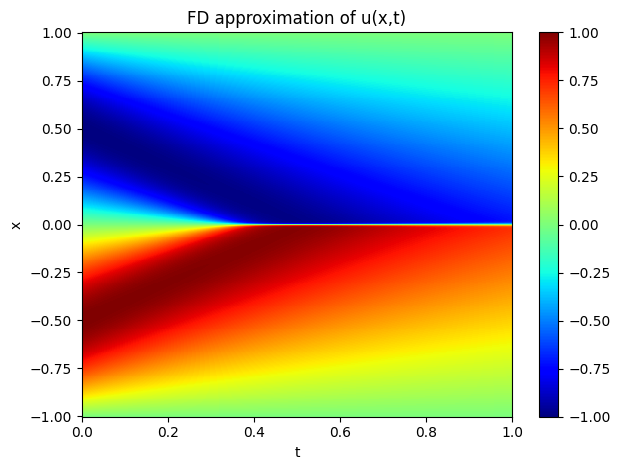
\includegraphics[width=300px]{images/FD_burgers_pde.png}
    \vspace{-1em}
    \caption{Finite difference approximation}
    \label{fd_burgers}
\end{figure}

Figure \ref{fd_burgers} shows the finite difference approximation of burgers' equation.

Let $\tilde{u}(x,t)$ be the approximated solution by the neural network. 
Furthermore, rearrange Burgers equation and define the following function
\begin{equation}
f(x,t) = \tilde{u}_t + \tilde{u} \tilde{u}_x - \nu \tilde{u}_{xx}
\end{equation}

Since we know that $f(x,t) = 0$, we can use this in our loss function, which is usually 
taken as the mean square error between the predicted and the true values.
\begin{equation}
MSE_{PDE} = \frac{1}{N_f} \sum_{i=1}^{N_f} \Big|f(x_i, t_i)\Big|^2
\end{equation}

Since $x\in [-1,1]$ and $t\in [0,1]$ then the collocation points are defined over 
the domain $(x_i, t_i) \in [-1,1] \, \times \, [0,1]$. $N_f$ is the number of collocation points.

Similarly, we can define the loss due to the initial and boundary points.
\begin{equation}
MSE_{0} = \frac{1}{N_0} \sum_{i=1}^{N_0} \Big| \tilde{u}(x_i, t=0) + \sin(\pi x_i)\Big|^2
\end{equation}
Where $N_0$ is the number of initial points.

\begin{equation}
\begin{aligned}
&MSE_{lb} = \frac{1}{N_{lb}} \sum_{i=1}^{N_{lb}} \Big| \tilde{u}(x=-1, t_i) \Big|^2 \\
&MSE_{rb} = \frac{1}{N_{rb}} \sum_{i=1}^{N_{rb}} \Big| \tilde{u}(x=1, t_i) \Big|^2
\end{aligned}
\end{equation}
Where $N_{lb}$ and $N_{rb}$ are the number of left boundary and right boundary points, respectively.

The loss function that we need to minimize is the sum of PDE, initial, and boundary losses. Therefore,
\begin{equation}
MSE = MSE_{PDE} + MES_{init} + MSE_{lb} + MSE_{rb}
\end{equation}

The neural network that was used to approximate the solution consists of 4 hidden layers
with each layer containing 32 neurons. The total number of collocation or training points is $N_f=2500$.
50 points from the spatial domain $[-1, 1]$ and 50 points from the temporal domain $[0, 1]$ and hence 
$N_f = 50 \times 50 = 2500$. Similar to the example of the diffusion problem, the optimizer that was used 
to minimize the loss function is the Adam optimizer with a learning rate of $10^{-4}$. Figure \ref{pinn_approx_burgers} 
shows the model approximation after training the neural network for 20000 iterations and Figure \ref{abs_difference_burgers}
shows the absolute difference between the FD solution and the PINN approximation.

\begin{figure}[H]
    \centering 
    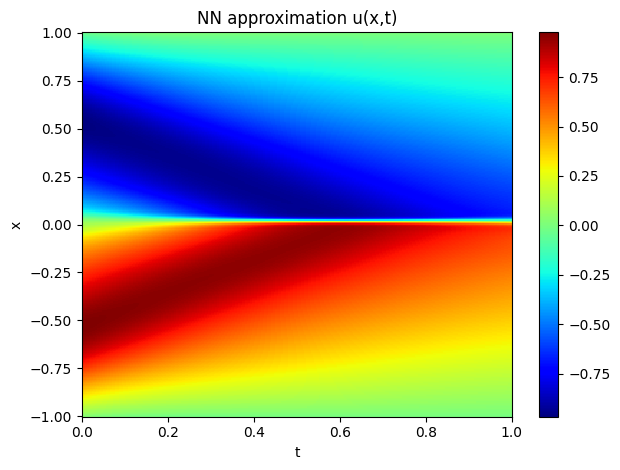
\includegraphics[width=300px]{images/NN_burgers_pde.png}
    \vspace{-1em}
    \caption{PINN approximation}
    \label{pinn_approx_burgers}
\end{figure}

\begin{figure}[H]
    \centering 
    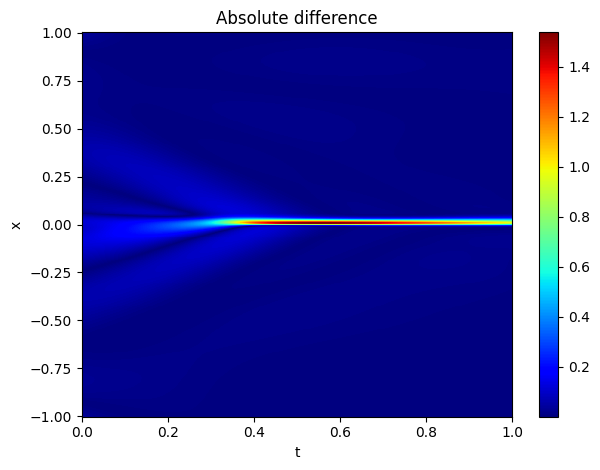
\includegraphics[width=300px]{images/abs_difference_burgers.png}
    \vspace{-1em}
    \caption{Absolute difference between FD and PINN}
    \label{abs_difference_burgers}
\end{figure}

Since we have not used the 
exact solution as our reference solution, we used the mean square error to compare the neural network approximation 
with reference solution and the mean square error is approximately $0.0122$. The code and the details of the simulation
are on \href{https://github.com/HashimAlSadah/MX-Project/blob/main/PINN/continuous_time_model/Continuous_time_PINN_Burgers_PDE.ipynb}
{GitHub}.

\subsection{Discrete-time model}
Instead of using the PDE immediately as we did in the case of the continuous model, 
we can perform a temporal discretization to the PDE using explicit/implicit Runge-Kutta method\cite{raissi2019physics}.
Let us consider the following general PDE.
\begin{equation}\label{main_discrete_time_eq}
\frac{\partial u(x,t)}{\partial t} = g[u(x,t)], \quad x \in \Omega, \quad t \in [0, T]
\end{equation}
Where $u(x,t)$ is the desired solution, and $g[\cdot]$ is a spatial differential operator.

Next, we apply a general Runge-Kutta scheme with q stages as with the following Butcher's tableau 
$$
\begin{array}{c|cccc}
c_1 & a_{11} & a_{12} & \dots & a_{1q} \\ 
c_2 & a_{21} & a_{22} & \dots & a_{2q} \\ 
\vdots & \vdots & \vdots & \ddots & \vdots \\ 
c_q & a_{q1} & a_{q2} & \dots & a_{qq} \\ 
\hline
& b_1 & b_2 & \dots & b_q
\end{array}
$$

This would result in the following equations as defined in \cite{iserles2009first}.
\begin{equation}\label{RK_discrt}
\begin{aligned}
& u_{n+c_i} = u_n + \Delta t \sum_{j=1}^{q} a_{ij} \, g[u_{n+c_j}] \qquad \text{for} \; i = 1, 2, \dots, q \\
& u_{n+1} = u_n + \Delta t \sum_{j=1}^{q} b_j \, g[u_{n+c_j}] 
\end{aligned}
\end{equation}
Where 
$$\: u_{n+c_j} = u(t+c_j \Delta t, x) \qquad \text{for} j = 1, 2, \dots, q$$ 

$u_{n + c_j}$ are the Runge-Kutta solutions or the intermediate solution and 
$u_{n+1}$ is the solution at the next step in time $u_{n+1} = u(t + \Delta t, x)$.
The neural network will take training points from the spatial domain as an input 
and will output the intermediate solutions along with the solution at the next time step $t_{n+1}$.
Therefore, the output layer will have $q+1$ neurons corresponding to the number of stages and the next 
solution. 
\begin{equation}\label{NN_RK_output}
NN_{out} \rightarrow [u_{n+c_1}(x), u_{n+c_2}(x), \dots, \ u_{n+c_q}(x), u_{n+1}(x)]
\end{equation}

Given the approximated output of the neural network, we can compute the ap\-prox\-i\-mat\-ed previous solution 
$u_{n}$ and the error between the approximated $u_n$ and the exact $u_n$, which is known.

We can rearrange (\ref{RK_discrt}), so that we have our neural network output on one side and the 
previous solution on the other side.

\begin{equation}\label{RK_discrt_rearranged}
\begin{aligned}
& u_n = u_{n+c_i} -  \Delta t \sum_{j=1}^{q} a_{ij} \, g[u_{n+c_j}] 
\qquad \text{for} \; i = 1, 2, \dots, q \\
& u_n = u_{n+1} - \Delta t \sum_{j=1}^{q} b_j \, g[u_{n+c_j}] 
\end{aligned}
\end{equation}

Since the previous steps in (\ref{RK_discrt_rearranged}) are the approximated, we will assign each one 
them a unique identifier as the following.

\begin{equation}\label{discrete_t_eqs}
\begin{aligned}
& u_n^{(i)} = u_{n+c_i} -  \Delta t \sum_{j=1}^{q} a_{ij} \, g[u_{n+c_j}] 
\qquad \text{for} \; i = 1, 2, \dots, q \\
& u_n^{(q+1)} = u_{n+1} - \Delta t \sum_{j=1}^{q} b_j \, g[u_{n+c_j}] 
\end{aligned}
\end{equation}
Therefore, the physics-informed output is 
\begin{equation}\label{phys_RK_output}
NN_{phys} \rightarrow [u_{n}^{(1)}, u_n^{(2)}, \dots, u_n^{(q)}, u_n^{(q+1)}]
\end{equation}

\textbf{Note:} (\ref{NN_RK_output}) is the neural network output without applying any equation 
and (\ref{phys_RK_output}) is the physics-informed output since we are applying (\ref{discrete_t_eqs})
to obtain (\ref{phys_RK_output}). 

For the purpose of implementation, it is better to write (\ref{discrete_t_eqs}) using vectors and 
matrix notation.
\begin{equation}
\begin{bmatrix}
    u_{n}^{(1)} \\ u_n^{(2)} \\ \vdots \\ u_n^{(q)} \\ u_n^{(q+1)}   
\end{bmatrix}
=
\begin{bmatrix}
u_{n+c_1} \\ u_{n+c_2} \\ \vdots \\ u_{n+c_q} \\ u_{n+1}
\end{bmatrix}
-
\Delta t
\begin{bmatrix}
    a_{11} & a_{12} & \dots & \dots & a_{1q} \\
    a_{21} & a_{22} & \dots & \dots & a_{2q} \\
    \vdots & \vdots & \vdots & \vdots & \vdots \\
    a_{q1} & a_{q2} & \dots & \dots & a_{qq} \\
    b_{1} & b_{2} & \dots & \dots & b_{q} \\
\end{bmatrix}
\begin{bmatrix}
g_1 \\ g_2 \\ \vdots \\ g_{q-1} \\ g_{q}
\end{bmatrix}
\end{equation}

Where 
$$g_j = g[u_{n+c_j}], \qquad  j = 1, 2, \dots, q$$

Finally, we define the loss function, which is the mean square error between the exact and the approximated 
solution of the previous step in time.
\begin{equation}
MSE_{n} = \frac{1}{N_x (q+1)} \sum_{j=1}^{N_x} \sum_{i=1}^{q+1} \Big| u_n^{(i)}(x_j) - u_n(x_j) \Big|^2
\end{equation}
Where $N_x$ is the number of nodes or training points from the domain $\Omega$ and $q$ is the number 
of stages of Runge-Kutta method.

\textbf{Note:} We have only defined a loss function for the inner points and not for the boundary
points since we have not specified the geometry of the problem and the type of boundary conditions.
However, the loss function for the boundary points $MSE_b$ can be defined depending on 
the problem's specifications and the total loss will be $MSE = MSE_n + MSE_b$ as we will see in the following 
example.  

After training the neural network or the model we should be able to predict the solution $u(x, t + \Delta t)$
at the next step in time $t_{n+1}$. To find the value of $u$ at $t_{n+2}$, we need to train the neural network
again using the approximation that we have acquired at $t_{n}$. In other words, we have to implement a time marching 
scheme. 

An advantage of this method is that we could approximate the solution at the last time step in time $T$ immediately
if we use an implicit Runge-Kutta. An implicit Runge-Kutta scheme with large number of stages will have a larger 
stability region and hence one can use a greater step size to obtain the solution at the final step in one shot. 
The same advantage can be a limitation in certain cases where we would like to observe how the simulated system 
evolves in time, which may requires us to compute the solution using a small step.
However, we can always use a time marching scheme to resolve this issue.

\subsubsection{Linear PDE example}
Consider the following diffusion equation 
\begin{equation}\label{diffusion_discrete_time}
\frac{\partial u(x,t)}{\partial t} = \frac{\partial^2 u(x,t)}{\partial x^2} - u(x, t),
\quad 0 < x < 1, \quad 0 < t  \le 1
\end{equation}

Subject to the following boundary and initial conditions
\begin{equation}
u(x = 0, t) = u(x= 1, t) = 0, \quad t \ge 0
\end{equation}
\begin{equation}
u(x, t=0) = sin(\pi x), \quad x \in [0, 1] 
\end{equation}

The exact solution is 
\begin{equation}
u(x,t) = sin(\pi x) e^{-(\pi^2 + 1)t}
\end{equation}

We write (\ref{diffusion_discrete_time}) in the form of (\ref{main_discrete_time_eq}) 
by defining the following differential operator
\begin{equation}
g[u(x,t)] = \frac{\partial^2 u(x,t)}{\partial x^2} - u(x, t)
\end{equation}

For this problem, we are going to apply an implicit Runge-Kutta with three stages with following
Butcher's tableau.
\begin{equation}
\begin{array}{c|ccc}
    0 & \frac{1}{9} &  \frac{-1-\sqrt{6}}{18} &  
    \frac{-1+\sqrt{6}}{18}\\[0.25em]
    \frac{3}{5} - \frac{\sqrt{6}}{10} & \frac{1}{9} & \frac{11}{45} + 
    \frac{7\sqrt{6}}{360} & \frac{11}{45} - \frac{43\sqrt{6}}{360} \\[0.25em]
    \frac{3}{5} + \frac{\sqrt{6}}{10} & \frac{1}{9} &
    \frac{11}{45} + \frac{43\sqrt{6}}{360} & \frac{11}{45} - \frac{7\sqrt{6}}{360}\\[0.25em]
    \hline \\[-1em]
    & \frac{1}{9} & \frac{4}{9} + \frac{\sqrt{6}}{26} &
    \frac{4}{9} - \frac{\sqrt{6}}{26}
    \end{array}
\end{equation}

Therefore, our linear system is 
\begin{equation}
\begin{bmatrix}
u_n^{(1)} \\ u_n^{(2)} \\ u_n^{(3)} \\ u_n^{(4)} 
\end{bmatrix}
=
\begin{bmatrix}
u_{n+c_1} \\ u_{n+c_2} \\ u_{n+c_3} \\ u_{n+1} 
\end{bmatrix}
-
\Delta t
\begin{bmatrix}
a_{11} & a_{12} & a_{13} \\
a_{21} & a_{22} & a_{23} \\
a_{31} & a_{32} & a_{33} \\
b_{1} & b_{2} & b_{3} \\
\end{bmatrix}
\begin{bmatrix}
g[u_{n+c_1}] \\ g[u_{n+c_2}] \\ g[u_{n+c_3}]
\end{bmatrix}
\end{equation}
Where 
$$
\text{NN}_{out} = [u_{n+c_1}, u_{n+c_2}, u_{n+c_3}, u_{n+1}]
$$
$$
\text{NN}_{phys} = [u_n^{(1)}, u_n^{(2)}, u_n^{(3)}, u_n^(4)]
$$

The loss function is defined as the following
\begin{equation}
MSE = MSE_n + MSE_b
\end{equation}
$MSE_n$ is the loss function for the points in the domain, $x \in (0, 1)$.
\begin{equation}
    MSE_n = \frac{1}{N_x  (q+1)}
    \sum_{j=1}^{N_x} \sum_{i=1}^{q+1} \,
    \Big| u^{(i)}_n(x_j) - u_n(x_j) \Big|^2
\end{equation}

$MSE_b$ is the loss function for the boundary points, $x=0$ and $x=1$.
\begin{multline}
MSE_b = \frac{1}{q} \left( \sum_{i=1}^{q} \Big| u_{n+c_i}(x=0) \Big|^2  \right)
+ \Big| u_{n+1}(x=0) \Big|^2 + \\
\frac{1}{q} \left( \sum_{i=1}^{q} \Big| u_{n+c_i}(x=1) \Big|^2  \right)
+ \Big| u_{n+1}(x=1) \Big|^2
\end{multline}
Where $N_x$ is the number of training points and $q = 3$ is the number of Runge-Kutta stages.

The neural network consists of 4 hidden layers and 64 hidden layers, and the optimizer used to
minimize the loss function is the limited-memory BFGS (LBFGS), which is quasi-Newton method since 
it approximates the Hessian matrix (the second partial derivative of the loss function). The time
marching scheme applies a time step of $\Delta t = 0.01$ to obtain a smooth approximation and the number
of training points is $N_x = 200$.

Figure \ref{exact_approximation_diffusion_RK} shows the neural network approximation and the exact solution 
and Figure \ref{abs_diff_disc_pinn_diffusion} shows the absolute difference between the exact and the approximated
solutions, which indicates a global error of the order $10^3$. The details of the simulation are on 
\href{https://github.com/HashimAlSadah/MX-Project/blob/main/PINN/discrete_time_model/Discrete_time_PINN_Diffusion_equation.ipynb}
{GitHub repository}.


\begin{figure}[H]
    \centering
    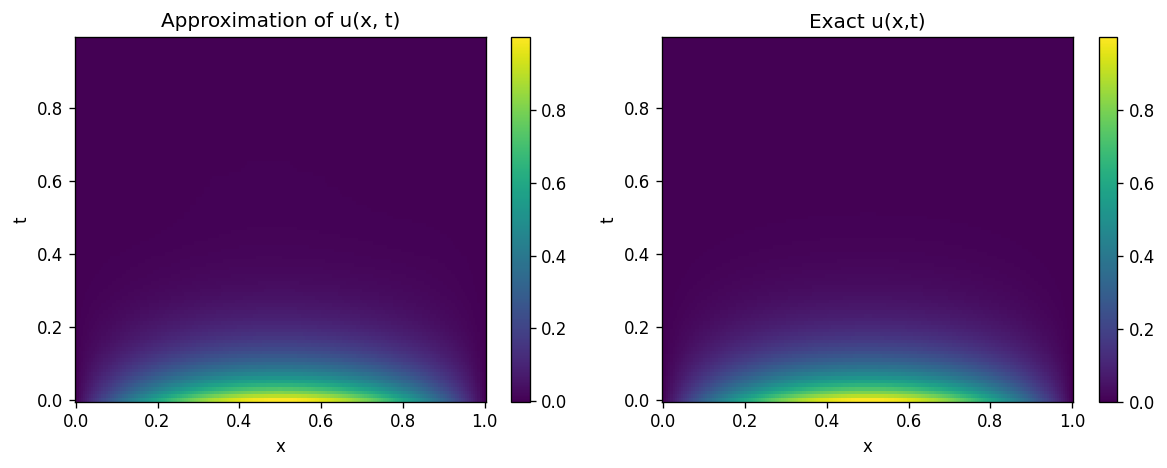
\includegraphics[width=420px]{images/diffusion_ex_app_dis_PINN.png}
    \vspace{-1em}
    \caption{Approximation and Exact solution of $u(x,t)$}
    \label{exact_approximation_diffusion_RK}
\end{figure}

\begin{figure}[H]
    \centering
    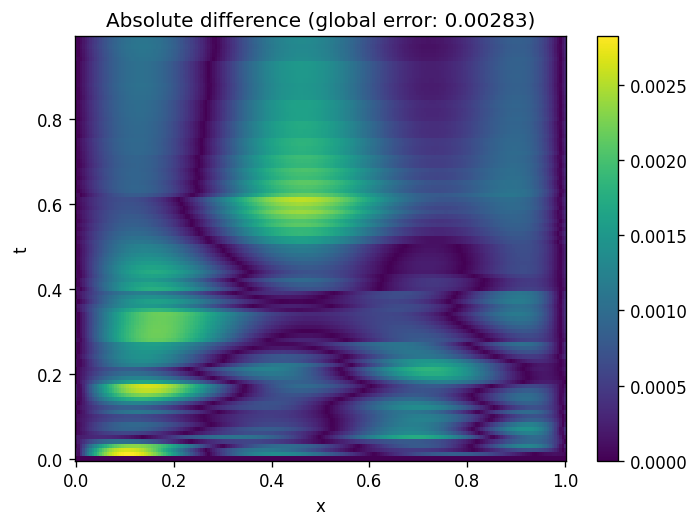
\includegraphics[width=250px]{images/abs_difference_disc_PINN_diffusion.png}
    \vspace{-1em}
    \caption{Absolute difference of $u_{exact} - u_{approx}$}
    \label{abs_diff_disc_pinn_diffusion}
\end{figure}

\clearpage
\section{PI-DeepOnet}
Physics Informed Deep Neural Operator (PI-DeepONet) is a DNN model for approximating  
the solutions of parametric partial differential equations (PDEs) where it incorporates 
physics informed knowledge in the architecture of the DeepONet model.
DeepONet is a neural network architecture used to learn
an operator between infinite dimensional function spaces. 

This section provides a concise overview of the DeepONet model architecture \cite{wang2021learning}, 
focusing specifically on the learning of solution operators for parametric Partial Differential Equations
(PDEs). The term "parametric PDEs" refers to PDE systems where certain parameters are permitted to vary 
within a specified range. These parameters could include factors such as the shape of the physical domain,
initial or boundary conditions, coefficients (constant or variable), and source terms. To address such 
problems comprehensively, let $(U, V, S)$ be a triplet of Banach spaces, and $N: U \times S \rightarrow
V$ be a differential operator, either linear or nonlinear. We examine parametric PDEs of the form 
$N(u, s) = 0$ \cite{wang2021learning} where $u \in U$ represents the parameters (input functions),
and $s \in S$ is the corresponding unknown solution to the PDE system. It is assumed that for any
$u \in U$, there exists a unique solution $s = s(u) \in U$ to the equation $N(u, s) = 0$ (subject to
appropriate initial and boundary conditions). Consequently, a solution operator $G: U \rightarrow S$ 
is defined as $G(u) = s(u)$. 

Following the original formulation by Lu et al. \cite{wang2021learning}, 
we represent the solution map $G$ using an unstacked DeepONet denoted as $G_{\theta}$, where $\theta$ 
encompasses all trainable parameters of the DeepONet network. As depicted in Figure \ref{DeepONet architecture}
DeepONet comprises two separate neural networks, known as the "branch net" and "trunk net", respectively.

\begin{figure}
    \centering
    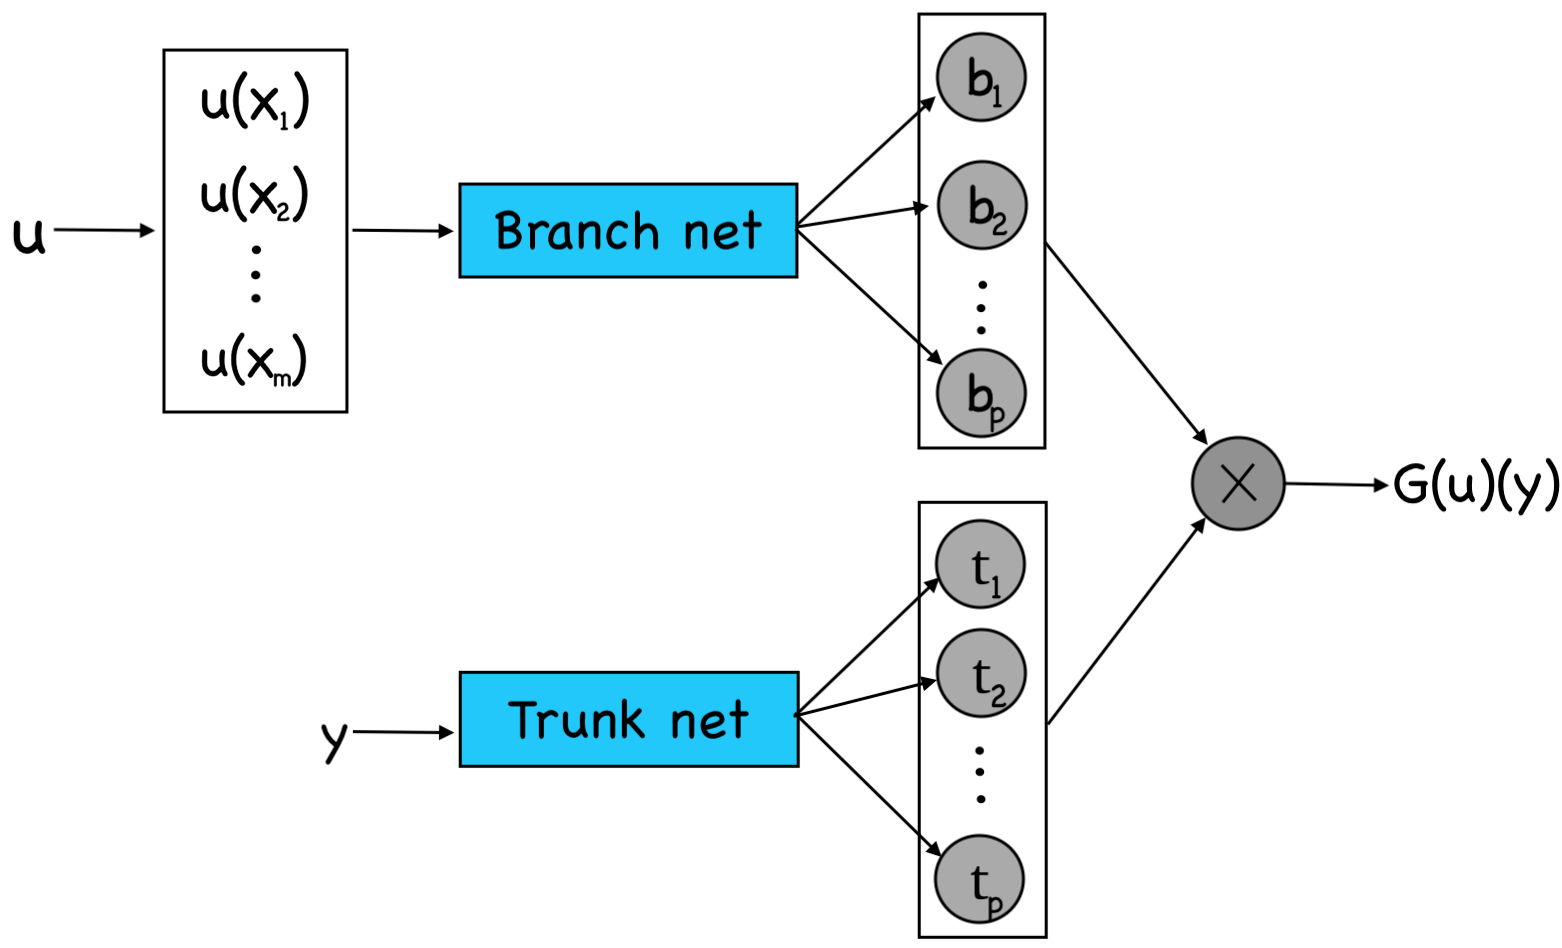
\includegraphics[width=300px]{images/DeepOnet.png}
    \caption{DeepONet architecture}
    \label{DeepONet architecture}
\end{figure}

The branch net takes $u$ as input and produces a feature embedding $[b_1, b_2, ..., b_q]^T \in \mathbb{R}^q$
as output, where $u = [u(x_1), u(x_2), ..., u(x_m)]$ denotes a function $u \in U$ evaluated at a set of 
fixed locations $\{x_i\}_{i=1}^m$. On the other hand, the trunk net accepts continuous coordinates $y$ as
inputs and generates a feature embedding $[t_1, t_2, ..., t_q]^T \in \mathbb{R}^q$ as output. The final 
output of the DeepONet is obtained by merging the outputs of the branch and trunk networks via a dot 
product. Specifically, the DeepONet prediction $G_{\theta}(u)(y)$ for a function $u$ evaluated at $y$
is expressed as:

\begin{equation}
G_{\theta}(u)(y) = \sum_{k=1}^{q} b_k(u(x_1), u(x_2), ..., u(x_m)) \cdot t_k(y),
\end{equation}

where $\theta$ represents the collection of all trainable weight and bias parameters in the branch and trunk networks. 
These parameters are optimized by minimizing the mean square error loss given by:
$$
\mathcal{L}_{ODE} = \frac{1}{m} \sum_{j=1}^{m}
\left(
-\frac{d^2 G_{\theta}(f)(p_j)}{dp^2} - f(p_j)
\right)^2_{p=x}
$$

Where $G_{\theta}(f)=u_{\theta}$ and $p_j$ is an input point to the trunk NN.

\subsection{IMPLEMENTATION}
We will consider the 1D Poisson equation as a study case to 
illustrate the implementation of the PI-DeepONet method. The 1D Poisson equation is given by:
$$
-\frac{d^2 u}{d x^2} = f(x), \quad 0 \le x \le 1
$$

Subject to the boundary conditions
$$
u(0) = u(1) = 0
$$
Where $f(x)$ is the forcing term. Our goal is to determine the function $u(x)$ for different
forcing terms$f(x)$. In other words, we are trying to determine an
operator $G$ such that $G:f \rightarrow u$.

The operator $G$ will be approximated by the branch neural network in the case of
the DeepOnet model, $G_{\theta} \approx G$. Where $\theta$ represents the parameter 
of the branch NN.
The model will consist of two neural networks, the branch NN and the trunk NN. 

\subsubsection{Branch Net}
In the branch net, we will consider the input to be the forcing term $f(x)$.
The input function space will be limited to a set of random polynomials of degree 3 
since it is not possible to implement an infinite function space. The space of polynomials
of degree 3 is given by 

\begin{equation}
    \mathcal{P}^n(x) =   a_0 + a_1 x + a_2 x^2 + \dots \dots + a_n x^n = \sum_{i=0}^{n} a_i x^i
\end{equation} 

Where $a_i \in \mathbb{R}$ and $n$ is the degree of the polynomial.

The branch net will take the forcing term $f(x)$ as input and output the approximated function $u(x)$.
In our work, we consider 100 different forcing terms $f(x)$ as the following 
  
\begin{equation}
branch_{in} =
\begin{pmatrix}
f_1(x_1) & f_1(x_2) & f_1(x_3) & \dots & f_1(x_{10})\\
f_2(x_1) & f_2(x_2) & f_2(x_3) & \dots & f_2(x_{10})\\
\vdots & \vdots & \vdots & \dots & \vdots\\
f_{100}(x_1) & f_{100}(x_2) & f_{100}(x_3) & \dots & f_{100}(x_{10})
\end{pmatrix}
\end{equation}

Which yields an output of: 
\begin{equation}
branch_{out} = \begin{pmatrix}
u^{(1)}_1 & u^{(1)}_2 & u^{(1)}_3 & \dots & u^{(1)}_m\\
u^{(2)}_1 & u^{(2)}_2 & u^{(2)}_3 & \dots & u^{(2)}_m\\
\vdots & \vdots & \vdots & \dots & \vdots\\
u^{(100)}_1 & u^{(100)}_2 & u^{(100)}_3 & \dots & u^{(100)}_m\\
\end{pmatrix}
\end{equation}

\begin{equation}
G_{\theta}:
\begin{bmatrix}
f_i(x_1) & f_i(x_2) & f_i(x_3) & \dots & f_i(x_{10})
\end{bmatrix}
\rightarrow
\begin{bmatrix}
u^{(i)}_1 & u^{(i)}_2 & u^{(i)}_3 & \dots & u^{(i)}_m
\end{bmatrix}
\end{equation}

for each $f_i(x)$ where $i=1, 2, 3, \dots, 100$
\begin{equation}
u_i(x) =
\begin{bmatrix}
u^{(i)}_1 & u^{(i)}_2 & u^{(i)}_3 & \dots & u^{(i)}_m
\end{bmatrix}
\end{equation}

$u_i(x)$ is not yet evaluated at any point. 
For the evaluation, we will use the output of the trunk neural network.

\subsubsection{Trunk Net}
The input to the trunk neural network are the points where we want to 
evaluate the target function $u(x)$ at, and we represent by the following column vector

\begin{equation}
trunk_{in} =
\begin{pmatrix}
p_1 \\
p_2 \\
\vdots \\
p_{100}
\end{pmatrix}
\end{equation}

\textbf{Note}:  We used $p$ instead of $x$, so there is no confusion with between these points and the sensor points.

Since $0 \le x \le 1$, then $0 \le p_j \le 1$ for $j=1, 2, 3, \dots 100$

The trunk neural network will map each point to a higher dimension and in this case, we 
require that the output dimensions of the branch and the trunk networks must be the same. 
Therefore, the output of the trunk neural network is the following.

\begin{equation}
trunk_{out} = \begin{pmatrix}
b^{(1)}_1 & b^{(1)}_2 & b^{(1)}_3 & \dots & b^{(1)}_m\\
b^{(2)}_1 & b^{(2)}_2 & b^{(2)}_3 & \dots & b^{(2)}_m\\
\vdots & \vdots & \vdots & \dots & \vdots \\
b^{(100)}_1 & b^{(100)}_2 & b^{(100)}_3 & \dots & b^{(100)}_m\\
\end{pmatrix}
\end{equation}


For each $p_j$ where $j=1, 2, 3, \dots, 100$,

\begin{equation}
\mathbf{NN}_{\text{trunk}}(p_j) = \begin{bmatrix}
b^{(j)}_1 & b^{(j)}_2 & b^{(j)}_3 & \dots & b^{(j)}_m
\end{bmatrix}
\end{equation}

\subsubsection{Evaluation}
To evaluate the output $u_i$ at the trunk points,
we take the dot product of the branch output and the trunk output and that is why we require the
output dimensions of both networks to be the same. For example,
to evaluate $G(f_i)$ at $p_j$ we perform the following operation

\begin{multline}
G_{\theta}(f_i)(p_j) = u_i(p_j) = \\ 
\begin{bmatrix}
u^{(i)}_1 & u^{(i)}_2 & u^{(i)}_3 & \dots & u^{(i)}_m
\end{bmatrix} \cdot 
\begin{bmatrix} 
b^{(j)}_1 & b^{(j)}_2 & b^{(j)}_3 & \dots & b^{(j)}_m
\end{bmatrix}
= \sum_{n=1}^{m} u^{(i)}_n b^{(j)}_n
\end{multline}

We are going to use only 1 hidden layer with 32 parameters for both the branch and trunk networks. 
Also, we will use LBFGS optimizer since it converges to the minimum faster.
\subsection{RESULTS}
We trained the model and are going to test it with $f(x)$ to be in the same space that we trained it on
and on functions outside the domain to see how general the model is.

\textbf{Case 1 - Constant}\\
For $f(x) = -1$ which is a simple case with an exact solution $u(x) = \frac{1}{2} (x^2 - x)$ we get the following results 

\begin{figure}[H]
    \centering 
    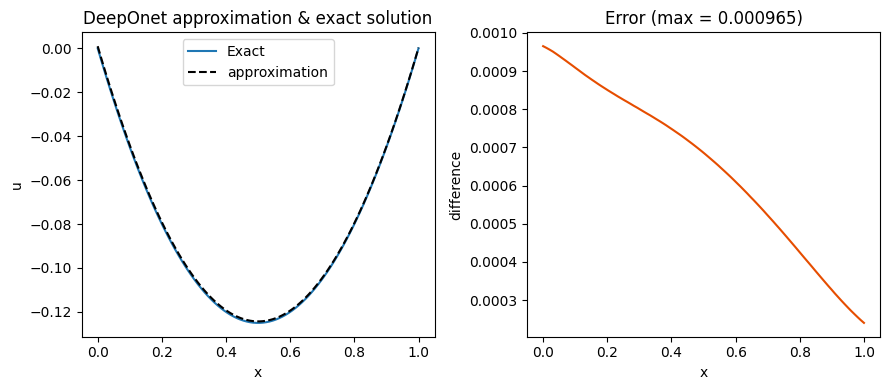
\includegraphics[width=\textwidth]{pideeponet_case1_result.png}
    \label{constant_f}
    \caption[figure1]{difference between the exact solution and the predicted solution for $f(x) = -1$}
\end{figure}

As we see in \ref*{constant_f}, the max error is very small, and the model 
was able to predict the solution very well.

\textbf{Case 2 - Quadratic}\\
In this case, we will consider the following forcing term
\[ f(x) = x + 3x^2 \] 
Which has an exact solution of 
\[u(x) = \dfrac{1}{6} x^3 - \dfrac{1}{4} x^4 + \dfrac{10}{24} x. \] 
The results are shown in the following figure

\begin{figure}[H]
    \centering 
    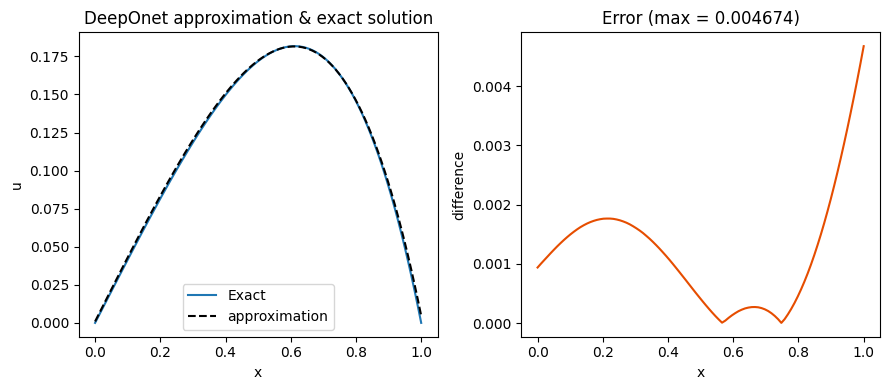
\includegraphics[width=\textwidth]{pideeponet_case2_result.png}
    \label{quadratic_f}
    \caption[figure2]{difference between the exact solution and the predicted solution for $f(x) = x + 3x^2$}
\end{figure}


\textbf{Case 3 - Out of Space Functions (Exponential)}\\
In this case, we will consider the following forcing term
\[f(x) = e^x\] 
Which has an exact solution of 
\[u(x) = - e^x +xe -x + 1\]
Since the forcing term is from a function space that the model hasn't been trained on, 
we expect the model to be less accurate. The results are shown in the following figure

\begin{figure}[H]
    \centering 
    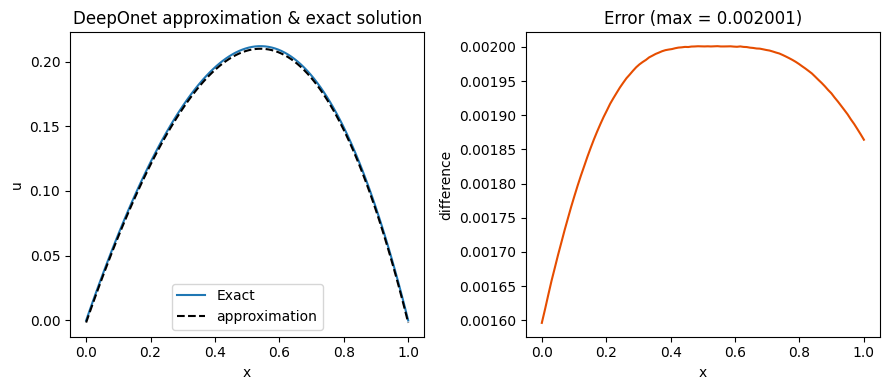
\includegraphics[width=\textwidth]{pideeponet_case3_result.png}
    \label{exp_f}
    \caption[figure3]{difference between the exact solution and the predicted solution for $f(x) = e^x$}
\end{figure}

\section{Conclusion}
The project shows the ability of Neural networks with different architecture
to approximate the solutions of PDEs. We explored the physics informed 
neural network (PINN) model to approximate the solutions for a nonlinear 
PDE (Burgers equation) and a linear PDE (diffusion equation) and the results 
match the reference solution with an acceptable accuracy. Furthermore, we 
implemented the two variations of PINN, which are the time-continuous model and
the time-discrete model, where the latter utilizes Runge-Kutta to discrete the 
temporal part of the PDE and thus reducing the number of input data to the neural network.
Finally, we looked into the physics informed DeepONet model, which approximates the solutions 
of parametric PDEs by learning a functional between two infinite dimensional function space. 
For this model, we only considered the time independent (one-dimensional) Poisson equation.
Despite the promise that Deep Learning methods show for approximating PDEs, they have certain 
limitations such as the need for a large amount of training points, especially for high dimensional
and multi-physics problems, the low accuracy of the approximated solution, and the long training time for 
neural network model.

\section*{Future Work}
Due to the time limit of this project we could not explore other interesting aspects 
of deep learning methods for approximating PDEs, so we suggest here few directions 
to continue the project.
\begin{itemize}
    \item Using PINNs to solve a multi-physics problems such as 
    the cavity flow problem represented by the Navier-Stocks equations or high dimensional ones 
    like many-body problems (for example, the simulation of electron gas).
    
    \item Implement the DeepONet to solve parametric PDEs such as approximating the 
    solution for burgers equation with different boundary or initial conditions.

    \item  Using deep learning methods to approximate the solution of PDEs with irregular 
    and complex geometry.

    \item Combining classical and deep learning approaches to create more robust methods.
\end{itemize}
 


%-----I will commment this page-------
%\section*{Outlines}
\begin{itemize}
    {\item \textbf{Literature Review} {\footnotesize(partially done)}}

    Searching the literature to get a better and clearer understanding of the theoretical 
    and the applied aspects of the topic. This will also help us to determine a relevant industrial problem.

    {\item \textbf{Establishing Connection with Industry}
    {\footnotesize(in progress)}}

    We are currently trying to contact potential companies and organization in order get an industrial 
    support and insight for the project. We are also, trying to find suitable industrial advisor 
    that has an experience in the related field.

    {\item \textbf{Reproducing Previous work} {\footnotesize(partially done)}}

    In order to deepen our understanding of the topic and have more confidence in our work and implementation, 
    we are trying to produce some the previous work in the literature.

    {\item \textbf{Solving the Main problem }}
    
    At this stage, we should be able to apply the skills and the methods that 
    we have searched about and developed to solve the industrial problem.

     {\item \textbf{Validating the Results }}

     After solving the problem, we need to validate our results by analyzing the obtained data.

    {\item \textbf{Demonstration}} 

    Preparing a demonstration to advertise or show the applicability of the project to solve actual problems. 
    This also includes preparing a poster, a report, and a presentation.

    {\item \textbf{Submitting the Project}} 
    
    At this stage, we should make a final review and corrections if necessary before the final submission. 
\end{itemize}
%--------------------------------------

%-------references------
\clearpage
\singlespacing
\bibliographystyle{plain}
\bibliography{ref.bib}
 

\end{document}
